% !TeX root = er.tex

\chapter{Swarm Robotics}\label{ch.swarm}

Factories use multiple robots to achieve goals such as painting and welding a car (Fig.\ref{fig.assemblyline}). The use of multiple robots shortens manufacturing time by performing different tasks simultaneously such as welding parts on both sides of a car. These tasks are typically designed to be independent with no close collaboration between the robots. Later, robots, especially mobile robots, were designed to collaborate with each other \emph{directly} to perform multiple actions simultaneously in different places.

Here are some examples of tasks that require multiple robots to collaborate:
\begin{itemize}
\item Manipulating large structural elements in buildings, as well as in environments that are hard for humans to access such as in space or underwater.
\item Performing a task through the collaboration of different types of robots: in a large-scale disaster, a flying drone can locate areas where victims are likely to be found, while a tracked robot on the ground searches these areas, focusing on places that may be hidden from aerial observation by trees or rubble.
\item Performing simultaneous measurements in different locations: measuring sound disturbances in different parts of a building, or monitoring pollution after an industrial accident. 
\end{itemize}
What is common to these situations is that multiple robots participate in performing a task and they need to coordinate with each other because they are acting on the same physical object even though they are not next to each other in the environment. 

Collaboration among robots can also be used to speed up the execution of a task by having several robots perform the task in parallel. Consider measuring pollution over a large area: a single robot can roam the entire area (like a robotic vacuum cleaner in an apartment), but the task will be accomplished much faster if multiple robots divide up the areas to be covered among themselves.

\section{Approaches to implementing robot collaboration}

There are two main approaches to the design of systems composed of multiple robots. The first is a \textit{centralized system}, where a central component (one of the robots or an external computer) coordinates all the robots and their tasks. The advantage of a centralized system is that it is relatively simple to implement. The main disadvantage is that it is difficult to expand because adding more robots adds processing load to the central station where all the intelligence is concentrated. In a centralized system, the robots themselves can be ``dumb,'' but most robots have significant computing power that is not well utilized in this architecture. Another serious disadvantage of a centralized system is that the central component is a single point of failure. If it stops working the entire system fails. In critical environments it is unacceptable to employ a system that is not robust under the failure of a single component.

If we look to the animal world, we see that many activities are \emph{distributed}, that is, independent individuals work together to achieve common goals of the entire population. Ants optimize their path to food sources not by depending on one ant to dispatch others to search and then to process the information returned, but by a distributed effort of the entire ant colony. Individual ants mark the ground with pheromones that are sensed by the other ants. If a few ants are eaten by a predator, the rest of the colony survives, as does the knowledge embodied in the locations of the pheromones. The efficiency and robustness of this approach was demonstrated in the algorithms in Chap.~\ref{ch.obstacle}.

\emph{Swarm robotics} is a distributed approach to robotics that tries to coordinate behavior by copying mechanisms inspired by the behavior of social animals. These mechanisms, often local and simple, allow a group to achieve global performance that could not be achieved by an individual on its own. Distributed systems have the following advantages:
\begin{itemize}
\item They are robust. Losing one out of ten robots only reduces the performance of the system by about ten percent instead of causing failure of the entire system.
\item They are flexible and scalable. The number of robots can be adapted to the task. If there are ten robots in the system but five are sufficient to perform the task, the other five can be assigned to other tasks, while if ten robots cannot perform the task efficiently, another ten can easily be added.
\end{itemize}
These advantages come at the cost of the effort required to design and implement coordination among the robots. In swarm robotics, as well as in nature, there are relatively simple coordination mechanisms that make distributed systems feasible.

This chapter presents two approaches to coordination in swarm robotics: \begin{itemize}
\item Information-based coordination (Sec.~\ref{s.swarm-info}), where the interaction is in the form of communications between robots. This can be either directly by explicitly passing electronic messages or indirectly by placing messages in the environment.
\item Physical coordination (Sec.~\ref{s.swarm-physical}), where individual robots interact at the mechanical level, either directly by exerting forces on each other or indirectly by manipulating a common object.
\end{itemize}

\section{Coordination by local exchange of information}\label{s.swarm-info}

Communications can be either global or local. Suppose that you receive a call from your friends and they inform you: ``We see an ice-cream store on the left.'' This \emph{global} information is useless unless they give you their current location. However, if you are walking side-by-side with them and one says: ``I see an ice-cream store on the left,'' from this \emph{local} information you immediately know the approximate location of the store and can easily locate it visually.

Inspired by nature, swarm robotics uses local communications within a distributed architecture. A few zebras on the outer edges of a herd look for predators and signal the others by sound or movement. Herding is a successful survival strategy for animals because local communications enables large numbers of animals to flee immediately upon detection of a predator by a small numbers of alert watchers.

\subsection{Direct communications}

\emph{Direct} local exchange of information is achieved when a friend talks to you. Animals don't talk but they do use sound as well as movement and physical contact to achieve direct local exchange of information. Robots implement direct local communications electronically (such as local WiFi or Bluetooth), or by transmitting and receiving light or sound. Alternatively, they can use a camera to detect changes in another robot such as turning on a light. 

Local communications can be either \emph{directional} or \emph{non-directional}. Radio communications such as Bluetooth is local (just a few meters) and generally the receiving robot does not attempt to determine the direction to the transmitting robot. Local directional communications can be implemented using a light source as the transmitter and a narrow-aperture detector or a camera as the receiver.

\subsection{Indirect communications}

\emph{Indirect} local communications refers to communications through a medium that can store a transmitted message for later access. The most familiar example is mail, either email or regular mail, where the transmitter composes the message and sends it, but the message remains at the server or the post office until it is delivered to the receiver who, in turn, may not access it immediately. Indirect communications in animals is called \emph{stigmergy}; animals leave messages by depositing chemical substances that other animals can sense. We mentioned the use of pheremones by ants; another example is the use of urine by a dog to mark its territory.

Chemical messages are hard to implement in robots, but robots can leave optical markings on the ground as we did in the algorithm simulating a colony of ants searching for a food source (Sect.~\ref{s.ant-like-algo}). There only one robot was used, but the algorithms could be easily implemented with multiple robots because it is the marking that is important, not the identity of the robot that created the marking.

Indirect communications can also be implemented by placing or manipulating objects in the environment. Robotic vacuum cleaners use \emph{beacons} that can be placed at the entrance of rooms that the robot should avoid. It is possible to conceive of beacons that record when a room has already been cleaned and this information is (indirectly) communicated to other vacuum cleaners.

\emph{Karel the Robot} is an environment used to teach programming. Commands move a virtual robot around a grid on a computer screen and the robot can deposit and sense ``beepers'' placed on squares of the grid (Fig.~\ref{fig.karel}).\footnote{The image is taken from the first author's implementation of Karel the Robot in Scratch (\url{https://scratch.mit.edu/studios/520857}).}

\begin{figure}
\begin{center}
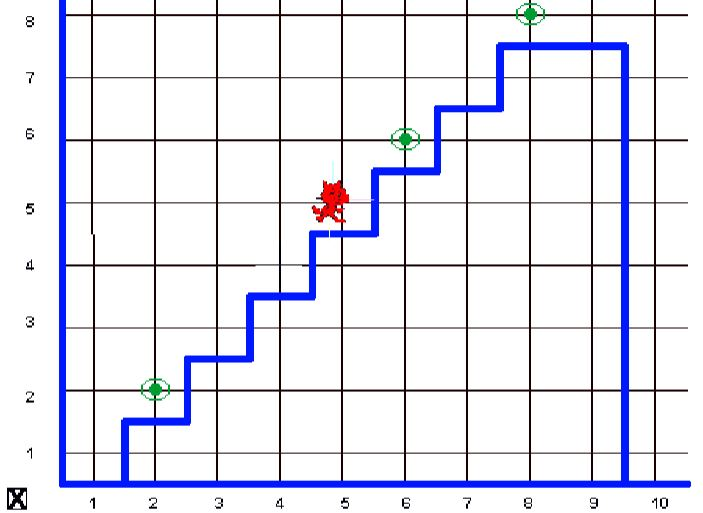
\includegraphics[width=.8\textwidth]{karel}
\end{center}
\caption{Karel the Robot implemented in Scratch; the green dots are the beepers}\label{fig.karel}
\end{figure}

Indirect communications when combined with manipulation can generate interesting patterns. Figure~\ref{fig.coll1} shows an environment filled with small objects and five mobile robots equipped with grippers. The robots follow a simple set of rules:
\begin{itemize}
\item If the robot finds an isolated object it picks the object up;
\item If the robot finds an isolated object but already holds one, it puts the new object down next to the one that was found;
\item The robot avoids walls and groups of several objects.
\end{itemize}
It seems that these rules will cause the robots to eventually place all the objects in groups of two, but this does not happen as shown in Fig.~\ref{fig.coll2}. The reason is that a group of objects \emph{seen from the side} can look like an isolated object, so an additional object is placed in the group. The result is that large groups of objects are assembled purely by indirect communication.

\begin{figure}
\begin{minipage}{.45\textwidth}
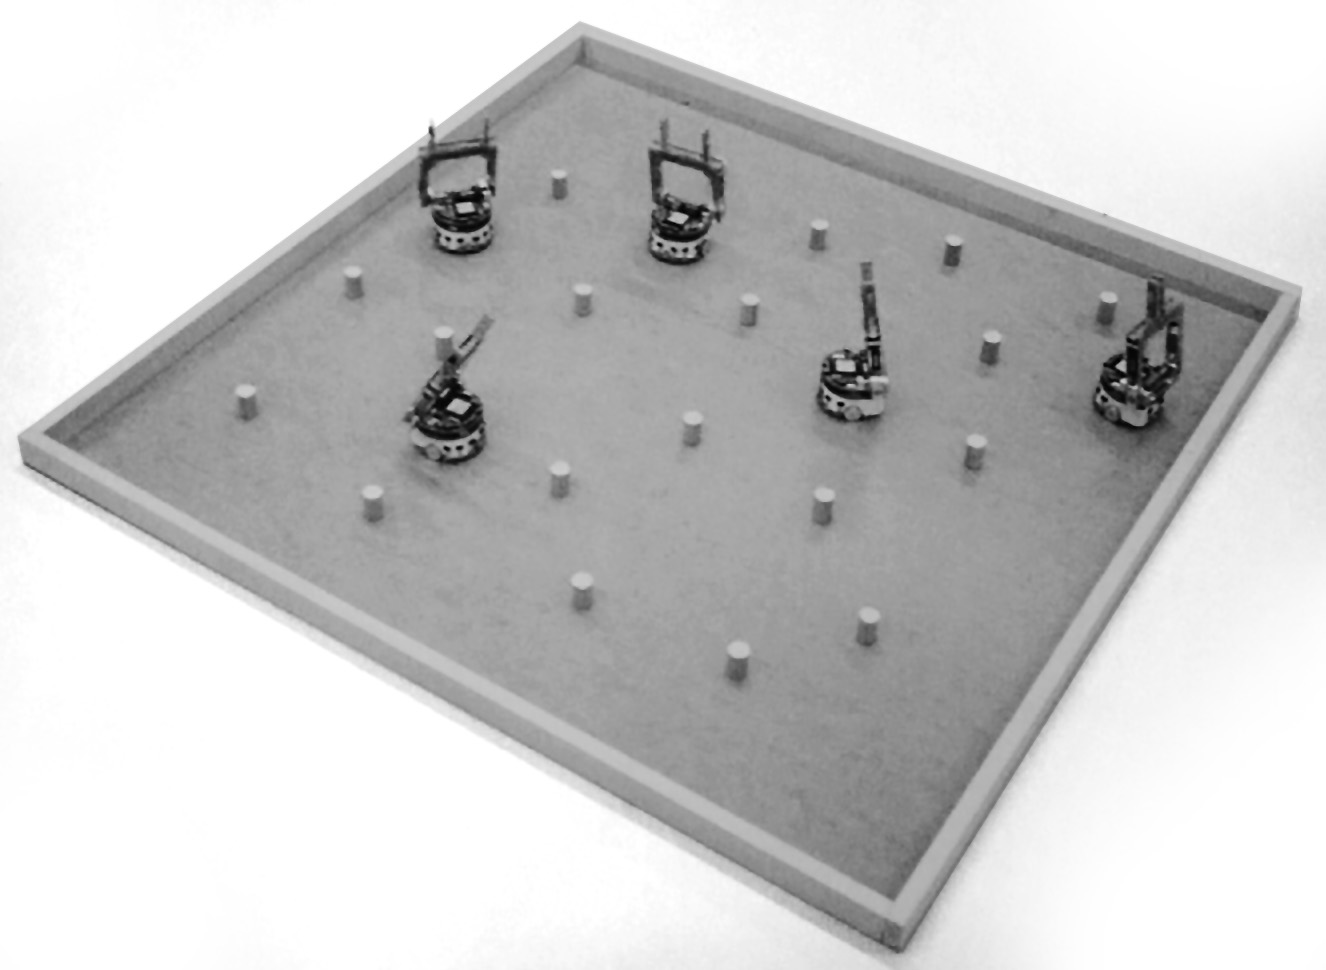
\includegraphics[width=.45\textwidth]{coll1}
\caption{Robôs garras em um ambiente repleto de pequenos objetos}
\label{fig.coll1}
\end{minipage}
\hspace{\fill}
\begin{minipage}{.45\textwidth}
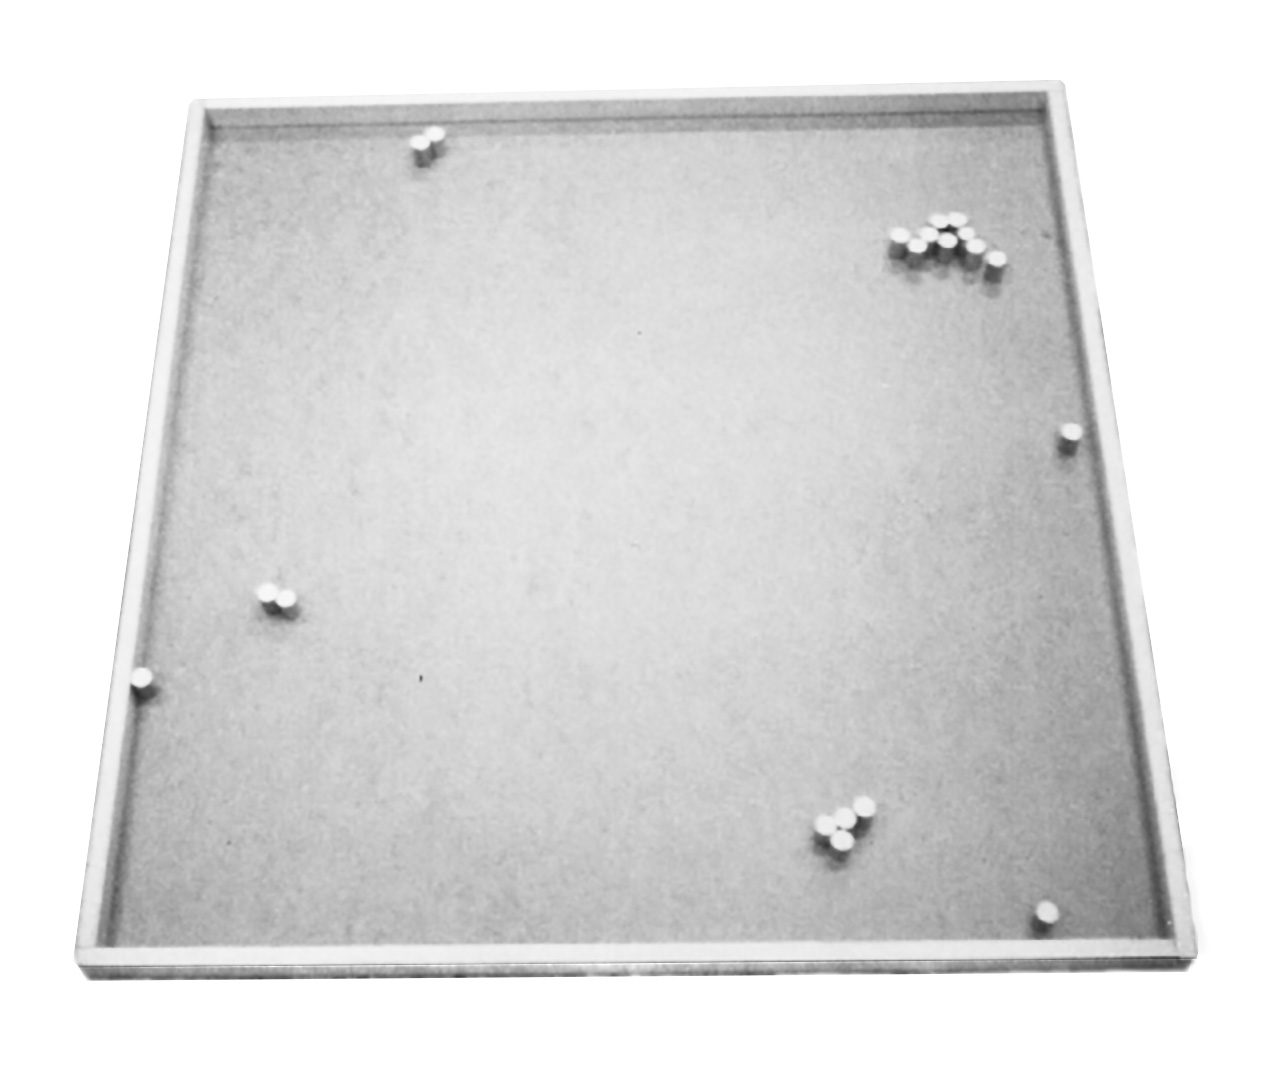
\includegraphics[width=.45\textwidth]{coll2}
\caption{Os objetos foram coletados em grupos}
\label{fig.coll2}
\end{minipage}
\end{figure}

%\begin{figure}
%\subfigures
%\begin{minipage}{\textwidth}
%\leftfigure{
%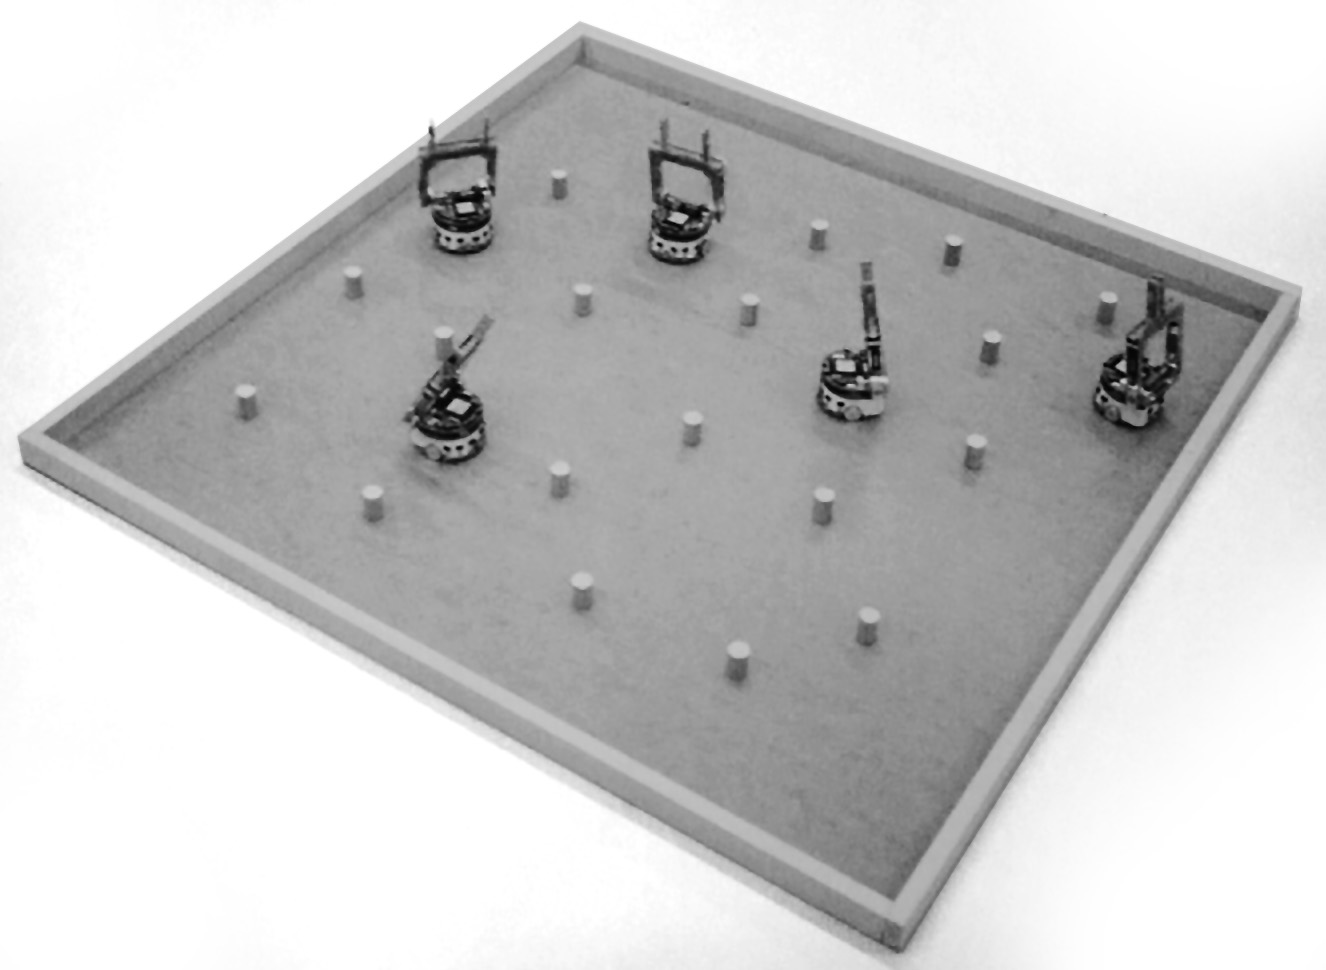
\includegraphics[width=.45\textwidth]{coll1}
%}
%\hspace{\fill}
%\rightfigure{
%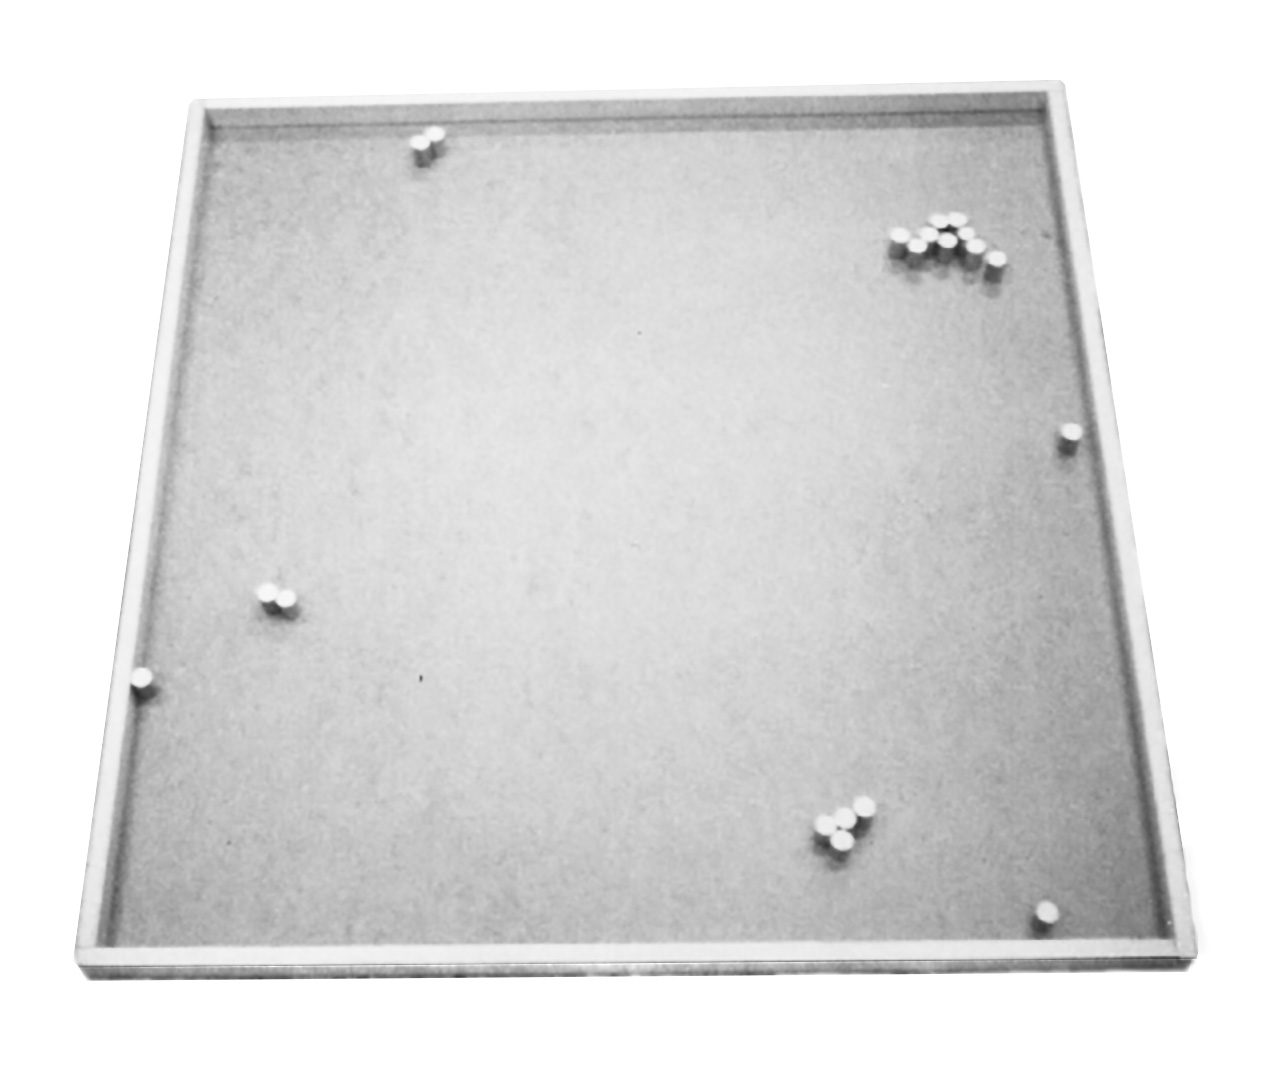
\includegraphics[width=.45\textwidth]{coll2}
%}
%\leftcaption{Gripper robots in an environment filled with small objects}\label{fig.coll1}
%\rightcaption{The objects have been collected into groups}\label{fig.coll2}
%\end{minipage}
%\end{figure}

\subsection{The BeeClust algorithm}


The BeeClust algorithm is a swarm algorithm inspired by the behavior of bees. It uses a distributed architecture and local communications to generate a global result. The BeeClust algorithm is based on the way that very young bees cluster around locations of optimal temperature in the darkness of their nest. They measure local temperatures and detect collisions with other bees.  The algorithm can be used by a swarm of robots to locate pollution; instead of measuring temperature, each robot measures some physical quantity that indicates levels of pollution. In time, the robots will come together in groups at locations of high levels of pollution.

Figure~\ref{fig.beeclust} shows a state machine implementing the algorithm. The robot moves randomly until it hits another robot, at which point it measures the temperature at the location of the collision. It waits at this location for a period of time proportional to the temperature that it found and then returns to moving randomly. When the robot moves it avoids obstacles such as walls. The algorithm uses what is perhaps the simplest form of communications: detecting a collision with another robot. The localized nature of the communications is essential for the correct functioning of the algorithm.

\begin{figure}
\begin{center}
\begin{tikzpicture}[node distance = 4cm and 5cm,align=left,minimum size=16mm,every loop/.style={min distance=16mm}]
% Nodes
\node[draw,circle] (moving) {\p{moving}};
\node[draw,circle] (waiting) [right=of moving] {\p{waiting}};
% Initial state arrow
\draw[->] (-15mm,10mm) to node [above left,yshift=-3mm] {\p{true} $\leadsto$ \p{fwd}} (moving);
% Transitions from moving
\path[->] (moving) edge [loop above] node [above,yshift=-4mm] {\p{collision with wall} $\leadsto$ \p{turn randomly, fwd}} ();
\path[->] (moving) edge node[above] {\p{collision with robot} $\leadsto$\\ \p{measure temperature,}\\\p{calculate waiting time}} (waiting);
% Transitions from waiting
\path[->,bend left=20] (waiting) edge node[below,yshift=3mm] {\p{wait expired} $\leadsto$ \p{turn randomly, fwd}} (moving);
\end{tikzpicture}
\end{center}
\caption{BeeClust algorithm}\label{fig.beeclust}
\end{figure}

Initially, the robots will collide at random places, but those that are in locations with higher temperatures will remain there for longer periods of time which in turn causes additional collisions. In the long term, most of the robots will form a cluster in the area with the highest temperatures. They collide with each other frequently since being in a crowd increases the number of collisions. Of course this mechanism can only work with a large number of robots that generate many collisions leading to numerous measurements and clustering. 

\subsection{The ASSISIbf implementation of BeeClust}

Within the ASSISIbf project, researchers at the University of Graz used Thymio robots to implement the BeeClust algorithm as part of research into the behavior of bees in a nest. The algorithm simulates a group of young bees in a cold circular arena, where two virtual sources of heat are placed on the right and on the left of the arena. Initially, only one of these sources of heat is active. The heat sources are simulated by two clusters of three robots at the edges of the arena (Fig.~\ref{fig.beeclust-demo}(a)).

\begin{figure}
\begin{center}
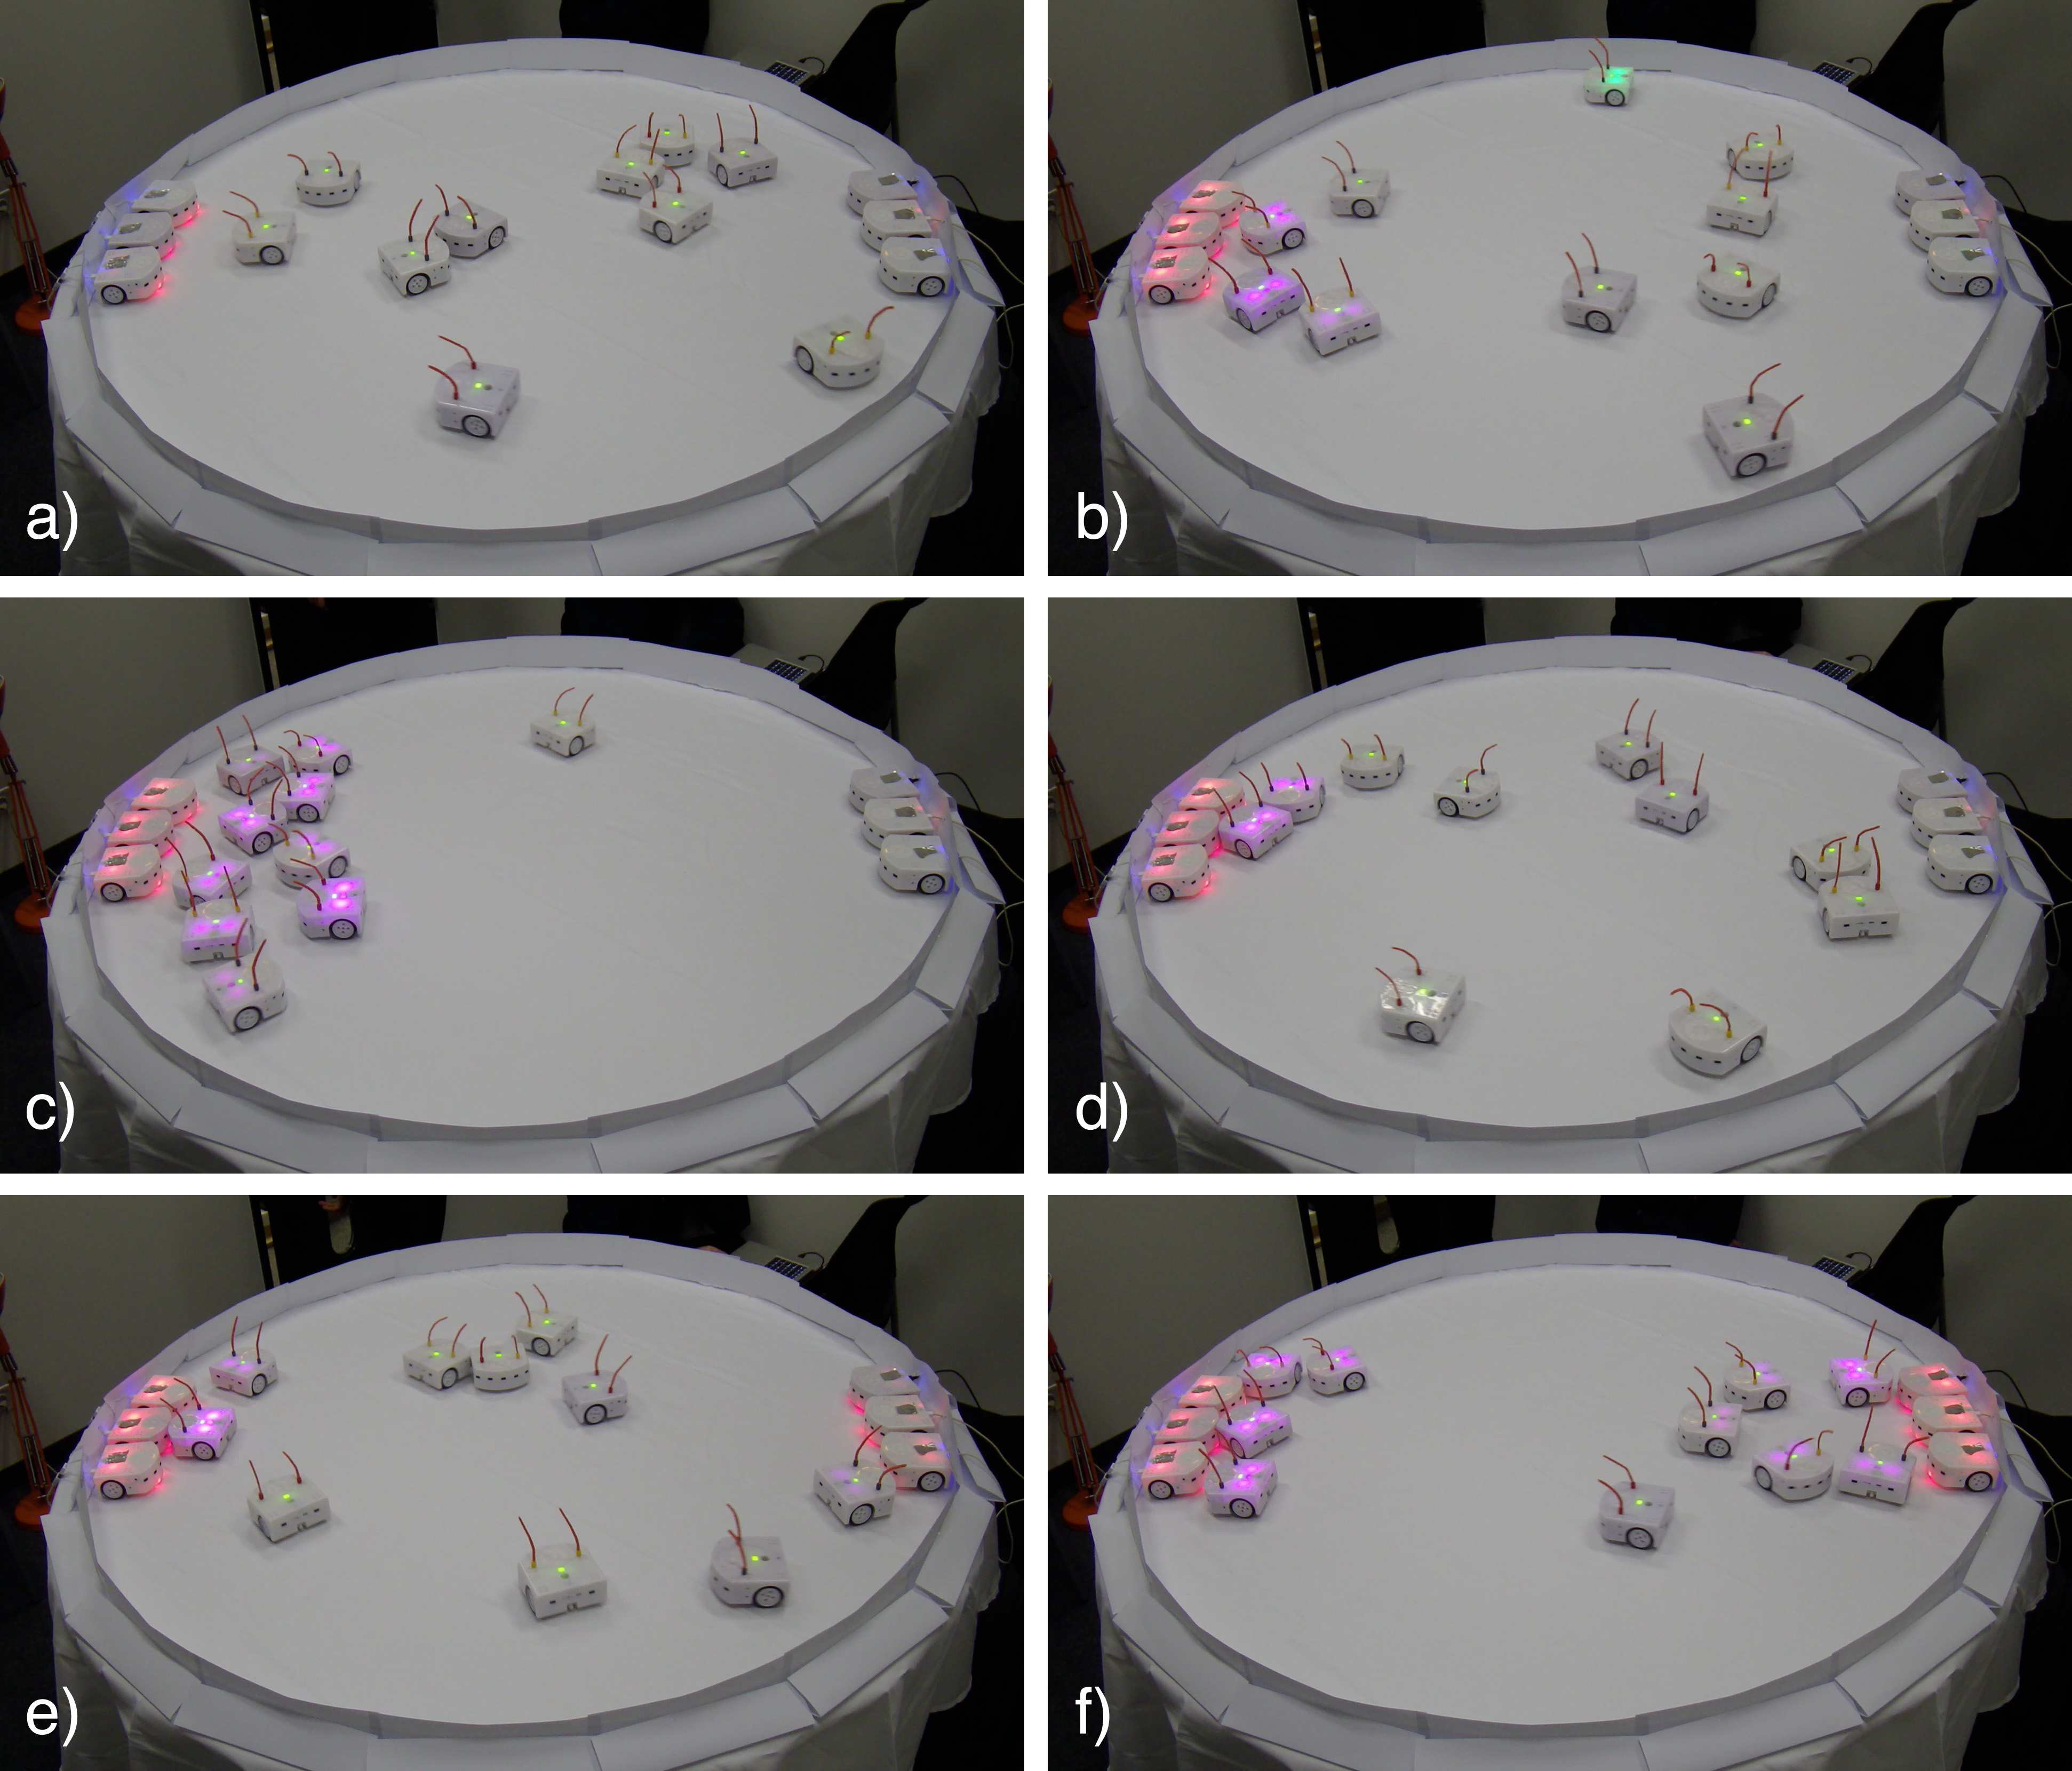
\includegraphics[width=\textwidth]{bee-clust}
\end{center}
\caption{BeeClust implementation. The photographs were taken at the following times (minutes:seconds) from the beginning of the experiment: a) 1:40, b) 2:30, c) 9:40, d) 12:40, e) 13:20, f) 21:10.}\label{fig.beeclust-demo}
\end{figure}

The three heat-emitting robots on the left side transmit their temperature. Bee-robots in their vicinity detect this signal and stop for a period of time proportional to the temperature. During their stay in this area they also transmit a temperature signal. Furthermore, if the heat-emitting robots detect nearby robots they increase their heat and transmit the new temperature. Figure~\ref{fig.beeclust-demo} shows the evolution of the behavior of the robots: (a) the initial state when the robots start moving and only the left temperature source is on; (b) the robots start clustering around the left source; (c) the highest level of clustering occurs. The bee-robots can leave the cluster, explore the environment and return to the cluster as shown in (d). This is caused by the random nature of the algorithm and is essential to prevent the system from being trapped in local minima. Figure~\ref{fig.beeclust-demo}~(e) shows the moment when the right source is also switched on. After about $21$ minutes the robots form two smaller clusters (f).

\begin{framed}
\act{BeeClust algorithm}{beeclust-swarm-act}
\begin{itemize}
\item Implement the BeeClust algorithm to cause a group of robots to cluster at the brightest location in a room.
\item Use three sensors: a light sensor to measure the ambient light, a sensor to detect other robots and a sensor to detect the limits of the arena.
\item Solution 1: Use proximity sensors to detect other robots and ground sensors to detect a line defining the limits of the arena.
\item Solution 2: Define the limits of the arena with a wall and use robot-to-robot communications to distinguish between robots and the wall. To avoid confusion do not use the same sensor to detect the other robots and the wall.
\end{itemize}
\end{framed}

\section{Swarm robotics based on physical interactions}\label{s.swarm-physical}

In Sect.~\ref{s.no-localization} we looked at a typical example of efficient swarm behavior: a colony of ants finding a path from their nest to a source of food. That example used indirect communications in the form of pheromones deposited on the ground. In this section we look at another form of swarm behavior that is mediated by physical interactions. We start with ants collaborating on the task of pulling a stick from the ground and a robotic version of this task. This is followed by a discussion of how forces exerted by several robots can be combined, demonstrated by a simple but clever algorithm called occlusion-based collective pushing.

\subsection{Collaborating on a physical task}

Figure~\ref{fig.real-ants-pulling} shows two ants extracting a stick from the ground for use in building a nest. The stick is embedded so deeply that one ant cannot extract it by itself. We want to design a robotic system to accomplish this task (Fig.~\ref{fig.robots-pulling}). Each robot searches randomly until it finds a stick. It then pulls on the stick as hard as possible. If it successfully extracts the stick, it takes it back to a nest; otherwise, since it has only partially extracted the stick, it waits until it feels that another robot is pulling harder and releases the stick. If no robot comes to its help for a period of time, the robot releases its hold and returns to a random search. This ensures that if there are more sticks than robots, the system won't deadlock with each robot trying to extract one stick and waiting indefinitely.
\begin{figure}
\begin{minipage}{.45\textwidth}
\includegraphics[width=.45\textwidth]{real-ants-pulling}
\caption{Formigas puxando um pau do chão}
\label{fig.real-ants-pulling}
\end{minipage}
\hspace{\fill}
\begin{minipage}{.45\textwidth}
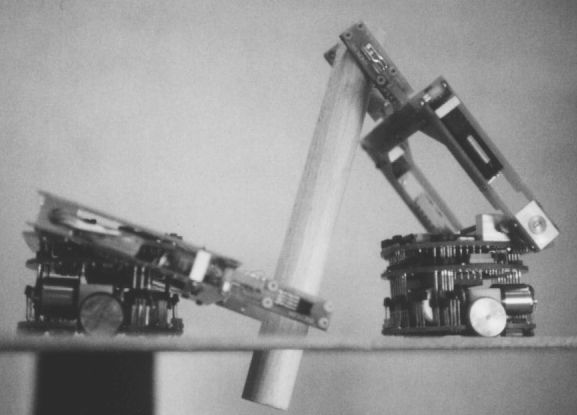
\includegraphics[width=.45\textwidth]{robots-pulling}
\caption{Robôs puxando um bastão do chão}
\label{fig.robots-pulling}
\end{minipage}
\end{figure}

%\begin{figure}
%\subfigures
%\begin{minipage}{\textwidth}
%\leftfigure{
%\includegraphics[width=.45\textwidth]{real-ants-pulling}
%}
%\hspace{\fill}
%\rightfigure{
%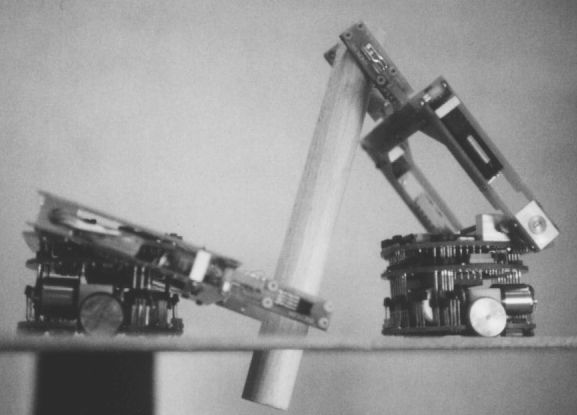
\includegraphics[width=.45\textwidth]{robots-pulling}
%}
%\leftcaption{Ants pulling a stick from the ground}\label{fig.real-ants-pulling}
%\rightcaption{Robots pulling a stick from the ground}\label{fig.robots-pulling}
%\end{minipage}
%\end{figure}

The finite state machine for this algorithm is shown in Fig.~\ref{fig.antspulling-FSM}. Although this behavior is simple and local, when applied by two robots it results in the extraction of the stick from the ground. The robot on the right in Fig.~\ref{fig.robots-pulling} pulls part of the stick as far as possible out of the ground using the maximum movement of its arm. When it detects that another robot has found the same stick and starts pulling, the first robot releases the stick to allow the second robot to extract it. By combining the physical capability of two robots with a simple specification of behavior, we achieve a result that neither of the robots could achieve alone.

\begin{figure}
\begin{center}
\begin{tikzpicture}[node distance = 2.5cm and 50mm,align=left,minimum size=14mm,every loop/.style={min distance=16mm}]
% Nodes
\node[draw,circle] (looking) {\p{searching}};
\node[draw,circle] (lifting) [right=of looking] {\p{lifting}};
\node[draw,circle] (to-home) [below=of lifting] {\p{bringing}\\\p{to nest}};
\node[draw,circle] (waiting) [below=of looking] {\p{waiting}};
% Initial state arrow
\draw[->] (-10mm,10mm) to node [above,yshift=0mm] {\p{true} $\leadsto$\\\p{fwd, set search timer}} (looking);
% Transitions from searching
\path[->] (looking) edge [loop left] node [below,yshift=-2mm] {\p{search timeout} $\leadsto$\\\p{turn randomly,}\\\p{fwd}} ();
\path[->] (looking) edge node[above,xshift=-2mm,yshift=-5mm] {\p{found} $\leadsto$  \p{grab and lift}} (lifting);
% Transitions from lifting
\path[->] (lifting) edge node[right] {\p{extracted} $\leadsto$\\ \p{go to nest}} (to-home);
\path[->,bend left=10] (lifting) edge node[above,yshift=4mm,xshift=3mm] {\p{max lift reached,}\\\p{not extracted} $\leadsto$\\\p{set wait timer}} (waiting);
% Transitions from to nest
\path[->,bend left=10] (to-home) edge node[left,yshift=-12mm,xshift=20mm] {\p{at nest} $\leadsto$} (looking);
% Transitions from waiting
\path[->,bend right=20] (waiting) edge node[right] {\p{wait}\\\p{timeout} $\leadsto$} (looking);
\path[->,bend left=20] (waiting) edge node[left,yshift=-8pt] {\p{another robot}\\\p{pulling} $\leadsto$ \\\p{release the stick}} (looking);
\end{tikzpicture}
\end{center}
\caption{Algorithm for distributed stick pulling}\label{fig.antspulling-FSM}
\end{figure}

\subsection{Combining the forces of multiple robots}

Fig~\ref{fig.pulling1} shows a differential-drive robot moving backwards (from left to right). It exerts a force $F_r$ that can be used to pull an object. Figure~\ref{fig.pulling2} shows two robots connected together so that they exert a force $F_{\sub{total}}$ when moving from left to right.

\begin{figure}
\begin{center}
\begin{tikzpicture}
\pic[scale=.7] at (0,0) { robot-side };
\draw[->,thick] (-1.6,.7) -- node[above left] {$F_r$} (1,.7);
\end{tikzpicture}
\caption{One robot pulling with a given force $F_r$}\label{fig.pulling1}
\end{center}
\end{figure}

\begin{figure}
\begin{center}
\begin{tikzpicture}[scale=.6]
\pic[rotate=-20,scale=.7] at (0,0) { robot-side };
\pic[rotate=-20,scale=.7] at (8.5,-.4) { robot-side };
\draw[->,thick] (-1.3,0.8) -- node[above left] {$F_{\textit{total}}$} (1,0.8);
\draw[fill,gray!60] (62mm,2mm) -- ++(70:7mm) -- ++(-20:10mm) -- ++(70:25mm) -- ++(-20:25mm) -- ++(-110:6.3mm) -- ++(160:19mm) -- ++(-110:26mm) -- cycle;
\path (13,-3) rectangle ++(1,-3mm);  % Dummy for extra space
\end{tikzpicture}
\caption{Two connected robots pulling with a given force $F_{total}$}\label{fig.pulling2}
\end{center}
\end{figure}

What is the relationship between $F_r$ and $F_{\sub{total}}$? There are three possibilities:
\begin{itemize}
\item $F_{\sub{total}} < 2 F_r$: The connected robots lose efficiency because the force they exert is less than that exerted by the two robots pulling separately.
\item $F_{\sub{total}} = 2 F_r$: The connected robots achieve the same efficiency as two separate robots.
\item $F_{\sub{total}} > 2 F_r$: The connected robots are more efficient that two separate ones.
\end{itemize}
Robots can achieve $F_{\sub{total}} > 2 F_r$, where the total force is greater than the sum of the forces exerted by the individual robots, because in some mechanical configurations the connected robots are more stable since their center of gravity better placed. 

\begin{framed}
\act{Pulling force by several robots.}{pulling_force}
\begin{itemize}
\item Connect two robots and check whether they exert a force that is less than, the same, or greater than twice that exerted by a single robot. You can connect the robots with a rigid connection as in Fig.~\ref{fig.pulling2} or with a flexible connection using string.
\item Measure $F_r$, the force exerted by a single robot, and then measure $F_{\sub{total}}$ the force exerted by the connected robots.
\item A \emph{dynamometer} (Fig~\ref{fig.dyna}) is the best instrument for measuring forces. If you do not have one available, you can use a cable, a pulley and weights (or a scale) as shown in Fig.~\ref{fig.scale}.
\item Change the orientation of the robots: pulling forwards instead of backwards. Does this change the result?
\item Experiment on different surfaces (hard ground, carpet, paper) and determine the effect of the surface on the resulting force.
\end{itemize}
\end{framed}

\begin{figure}
\begin{center}
\begin{tikzpicture}[scale=.8]
% Table
\draw[fill,gray] (-6,-7.2mm) rectangle +(12,2mm);
\draw[fill,gray] (-5,-7.2mm) rectangle +(4mm,-4mm);
\draw[fill,gray] (5,-7.2mm) rectangle +(4mm,-4mm);
% Robot
\pic[scale=.6] at (0,0) { robot-side };
\draw[->,thick] (3.7,.7) -- node[above] {$F_r$} (6,.7);
% Attachment
\draw (-3,8mm) rectangle +(2,4mm);
\draw (-1,1) -- (0,1);
% Spring
\draw (-20mm,14mm) -- (-50mm,14mm) -- (-50mm,6mm) -- (-20mm,6mm);
\draw (-50mm,10mm) -- (-60mm,10mm);
\draw (-50mm,10mm) -- ++(2mm,2mm) -- ++(2mm,-4mm) -- ++(2mm,4mm)  -- ++(2mm,-4mm) -- ++(2mm,4mm)  -- ++(2mm,-4mm) -- ++(2mm,4mm)  -- ++(2mm,-4mm) -- ++(2mm,4mm)  -- ++(2mm,-3mm);
\end{tikzpicture}
\caption{Measuring the force with a dynamometer}\label{fig.dyna}
\end{center}
\end{figure}

\begin{figure}
\begin{center}
\begin{tikzpicture}
% Table
\draw[fill,gray] (-2,-9mm) rectangle +(8,2mm);
\draw[fill,gray] (-1,-9mm) rectangle +(4mm,-15mm);
\draw[fill,gray] (5,-9mm) rectangle +(4mm,-15mm);
% Robot
\pic[scale=.6] at (0,-2.7mm) { robot-side };
\draw[->,thick] (3,.3) -- node[above] {$F_r$} (6,.3);
% Attachment
\draw[fill,gray!80] (-3,1mm) circle[radius=3mm];
\draw (-2.9,1mm) -- (-3.1,1mm);
\draw (-3,0mm) -- (-3,2mm);
\draw (-3,.4) -- (0,.4);
\draw (-33mm,2mm) -- ++(0,-19mm);
\draw[fill,gray!80] (-35mm,-16mm) rectangle +(4mm,4mm);
\draw (-40mm,-24mm) rectangle +(14mm,8mm);
\draw (-33mm,-20mm) circle[radius=3mm];
\draw[->] (-33mm,-20mm) -- +(30:3mm);
\end{tikzpicture}
\caption{Measuring the force with a weight and a scale}\label{fig.scale}
\end{center}
\end{figure}

\subsection{Occlusion-based collective pushing}

Let us consider another example of combining the force of multiple robots. Instead of a physical link as in Fig.~\ref{fig.pulling2}, we use many simple robots to push an object, imitating a group of ants. Again, the advantages of a distributed system are flexibility---engaging just the resources needed for the task---and robustness---if one robot fails, the object might move a bit slower but complete failure of the task does not occur. These advantages come at the cost of additional resources and the complexity of implementing coordination among the robots.

Figure~\ref{fig.swarm-pushing} shows a group of small robots pushing a large object represented by the circle towards a goal. One approach would be to determine the direction to the goal, to share this information among all the robots and to have each robot compute the direction it should push. This is not as simple as it may appear since a simple robot might not be able to determine its absolute position and heading.

A swarm robotics approach is called \emph{occlusion-based pushing}, which assumes that the robots have only local knowledge, not global knowledge of what the other robots are doing. The robots are able to determine whether they can detect the goal or not. For example, a bright light could be mounted on the goal and the robots equipped with a light sensor. 

\begin{figure}
\begin{center}
\begin{tikzpicture}[scale=1.1]
\node[circle,draw,thick] (center) at (0,0) [minimum size=40mm] {};
\coordinate (goal) at (6,1.5);
\draw[fill] (goal) circle [radius=1pt];
\draw[->,shorten >= 50mm] (0,0) -- (goal);
\node at (6.5,1.5) {\p{goal}};
% Use negative shorten arrow trick to extend the tangent lines
\draw[shorten >= -50mm] (goal) -- (tangent cs:node=center, point={(goal)}, solution=1);
\draw[shorten >= -50mm] (goal) -- (tangent cs:node=center, point={(goal)}, solution=2);
% Draw the pushing robots
\foreach \angle/\x/\y in { 0/0mm/0mm, -20/2mm/10mm, -40/7mm/18mm, 20/2mm/-10mm, 40/7mm/-18mm, 60/14mm/-22mm } {
  \pic[rotate=\angle,scale=0.3] at (\x-24mm, \y) { robot };
  \draw[->] (\x-24mm,\y) -- +(\angle:8mm);
}
% Draw the non-pushing robots
\pic[rotate=-80,scale=0.3] at (0mm, 28mm) { robot };
\path[->,bend right=40,red,thick] (0mm,28mm) edge (8mm,26mm);
\pic[rotate=60,scale=0.3] at (8mm, -28mm) { robot };
\path[->,bend left=30,red,thick] (8mm,-28mm) edge (16mm,-24mm);
\pic[rotate=-120,scale=0.3] at (30mm, 10mm) { robot };
\path[->,bend right=50,red,thick] (30mm,10mm) edge (36mm,4mm);
\end{tikzpicture}
\end{center}
\caption{Occlusion based coordination: straight black arrows for the robots pushing the object and curved red arrows for the robots searching for an occluded position}\label{fig.swarm-pushing}
\end{figure}

Figure~\ref{fig.FSM-swarm-pushing} shows the finite state machine for this algorithm. The robots search for the object; when they find it they place themselves perpendicular to the surface and push (straight black arrows). This could be implemented using a touch sensor or a proximity sensor. The robots continue to push as long as they \emph{do not} detect the goal. If they do detect the goal, they stop pushing, move away (curved red arrows) and commence a new search for an occluded position where they resume pushing. The result is that the vector sum of the forces exerted by the robots is in a direction that moves the object toward the goal. The occlusion algorithm leads to the task being performed without a central control unit and even without inter-robot communications.

\begin{figure}
\begin{center}
\begin{tikzpicture}[node distance = 4cm and 5cm,align=left,minimum size=16mm,every loop/.style={min distance=16mm}]
% Nodes
\node[draw,circle] (searching) {\p{searching}\\\p{for object}}; and their fit to the required performances of the system.
\node[draw,circle] (pushing) [right=of searching] {\p{pushing}};
% Initial state arrow
\draw[->] (-5mm,12mm) to node [above left,yshift=-2mm,xshift=6mm] {\p{true} $\leadsto$\\\p{move randomly}} (searching);
% Transitions from searching
\path[->,bend left=30] (searching) edge node [above,yshift=-4mm] {\p{object found and goal occluded} $\leadsto$\\\p{push object}} (pushing);
% Transitions from pushing
\path[->] (pushing) edge [loop right] node[below,xshift=-2mm] {\p{goal occluded} $\leadsto$} (pushing);
\path[->,bend left=30] (pushing) edge node[below,yshift=4mm] {\p{goal visible} $\leadsto$\p{move randomly}} (searching);
\path[->] (pushing) edge node[above,yshift=-6mm] {\p{object lost} $\leadsto$\p{move randomly}} (searching);
\end{tikzpicture}
\end{center}
\caption{Algorithm for occlusion-based coordination}\label{fig.FSM-swarm-pushing}
\end{figure}

\begin{framed}
\act{Total force}{total-force}
\begin{itemize}
\item Consider the configuration shown in Fig.~\ref{fig.total-force}. Robot $1$ is pushing an object at a $45^{\circ}$ angle with force $f_1$, robot $2$ is pushing horizontally with force $f_2$ and robot $3$ is pushing vertically with force $f_3$. Show that the $f_{\sub{total}}$, the total force on the object, has magnitude:
\[
\sqrt{\left(f_2+\frac{f_1}{\sqrt{2}}\right)^2+\left(f_3-\frac{f_1}{\sqrt{2}}\right)^2}\,.
\]
in the direction:
\[
\alpha = \tan^{-1} \frac{2f_3-\sqrt{2}f_1}{2f_2+\sqrt{2}f_1}\,.
\]
\item Compute the magnitude and direction of $f_{\sub{total}}$ for various values of the individual forces. If $f_1=f_2=f_3=1$, the magnitude is $\sqrt{3}$ and the direction is $9.7^{\circ}$. If $f_1=f_2=1$, what must $f_3$ be so that $\alpha=45^{\circ}$?
\item Use three robots to implement this configuration and check that the object moves in the computed direction.
\end{itemize}
\end{framed}


\begin{figure}
\begin{center}
\begin{tikzpicture}[scale=1.2]
\draw[fill] (0,0) circle [radius=4pt];
\draw[->] (-3,0) -- node[above,near start] {$f_2$} (-4pt,0);
\draw[->] (0,-2) -- node[left,near start] {$f_3$} (0,-4pt);
\draw[->] (-45:-3) -- node[above,near start,yshift=4pt] {$f_1$} (-2pt,2pt);
\draw (-10mm,0) arc (180:135:10mm) node[midway,xshift=-3mm,yshift=1mm] {$45^{\circ}$};
\draw[dashed] (0,0) -- (3,0);
\draw[->] (0,0) -- node[above,near end,xshift=-1mm] {$f_{\sub{total}}$} (20:3);
\draw (15mm,0) arc (0:20:15mm) node[right,midway] {$\alpha$};
\end{tikzpicture}
\caption{The total force from three robots}\label{fig.total-force}
\end{center}
\end{figure}

\begin{framed}
\act{Occlusion-based pushing}{occulsion-swarm}
\begin{itemize}
\item Place three robots around an object and place a goal some distance away from the robot. Implement a mechanism for the robots to determine the direction to the goal, for example, attach a light to the goal or place the goal at the lowest point of an inclined surface.
\item Implement a mechanism that enables the robots to distinguish between the object and the boundary of the surface on which they move. For example, use a black tape on the surface for its boundary and detect the object using proximity sensors.
\item Implement a mechanism so that robots do not push each other. One method would be to use a color sensor and attach colored tape to the robots.
\item Implement the occlusion-based pushing algorithm.
\item Discuss whether occlusion-based pushing could be used in three dimensions, for example, underwater robots pushing an object.
\end{itemize}
\end{framed}

\section{Summary}

Swarm robotics uses multiple robots in a distributed architecture to perform a task. With a distributed architecture, the system is robust to the failure of individual robots and flexible in its ability to add or remove robots as the scale of the task changes. A distributed architecture can perform tasks that individual robots cannot, as we saw in the examples of robots combining forces. Finally, multiple robots can act simultaneously at different locations that are far from each other. These advantages come at a price: the increased cost of the multiple robots, the complexity of the coordination mechanisms that must be implemented, and in some cases the loss of performance due to the overlap between the action of different robots. 


\section{Further reading}

An overview of collective robotics is given in \cite{kernbach2013handbook} and the collection~\cite{sahin2005} focuses on swarm robotics. For the specific projects presented in this chapters see:
\begin{itemize}
\item Karel the Robot~\cite{karel}.
\item BeeClust~\cite{bodi2012interaction} and~\cite{Schmickl2009}.
\item ASSISIbf~\cite{schmickl2013assisi} and \url{http://assisi-project.eu}.
\item Physical interaction (pulling a stick)~\cite{Ijspeert2001}.
\item Occlusion-based transport~\cite{chen2013strategy} and \cite{gross2015}.
\end{itemize}
